\section{Topic models}
%02 12 2014

Topic models are algorithms for discovering the main themes that pervade a large and otherwise unstructured collection of documents.
The idea behind probabilistic modelling is to treat data as observations arising from a generative probabilistic process that includes hidden variables. This hidden layer of organization, whereby observations are structured, is what we want to find in the data. 
In the field of text mining the hidden variables reflect the thematic structure (that we do not have access to) of a collection of text documents composed by words. In our case the hidden variables represent the unknown activity routines that a subject performs during a day.
In a text document what is observed are the words. We, instead, observe a set of variables that are related to the activities of daily living performed by a subject during several days.

%Other possible version
%In the field of text mining the hidden variables reflect the thematic structure (that we do not have access to) of a collection of text documents composed by words. In our case the hidden variables represent the unknown activity routines that link together activity primitives like walking, sitting standing that a subject performs during a day. 
%In a text document what is observed are the words. Observing activity primitives in patients is tricky since the subjects should be asked to annotate what he or she does during the day or activity primitives should be recognized from measurable variables like limbs accelerations. This introduce errors that could propagate in the routine discovery.
%We, instead, observe a set of variables that are related to the activities of daily living performed by a subject during several days.

Following this preamble the intuition behind the use of the Latent Dirichelet Allocation (LDA) in activity routine discovery is that each day is a mixture of thematically coherent activities (routines) as a text document is a mixture of thematically coherent terms (topics). %exhibits
The graphical model for LDA is provided in Fig.~\ref{fig:LDA_model}.

%%%%%%%%%%%%%%%%%%%%%%%%%%%%	FIGURE TOPICMODEL		%%%%%%%%%%%%%%%%%%%%%%%%%%%%
\begin{figure}[ht]
\centering
    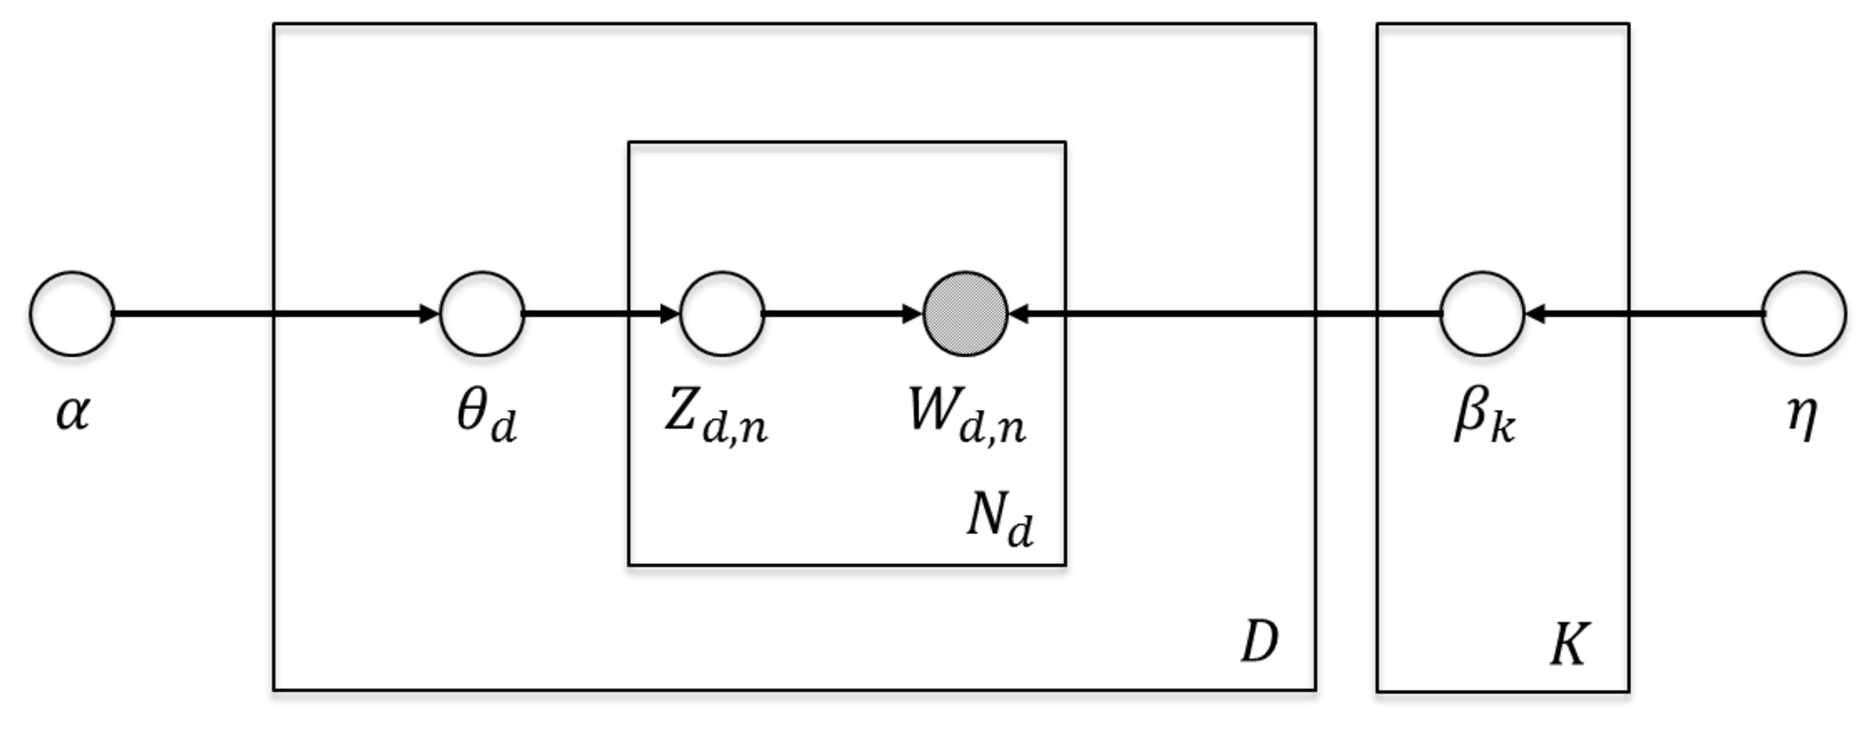
\includegraphics[width=.40\textwidth]{figure/eps/LDA_model.eps}
  \caption{Graphical model for LDA.Observations: words-documents.
Hidden structure: topjc structure, topics per document topic distributio, and the per document per word topic assignments.}\label{fig:LDA_model}
\end{figure}
%%%%%%%%%%%%%%%%%%%%%%%%%%%%%%%%%%%%%%%%%%%%%%%%%%%%%%%%%%%%%%%%%%%%%%%%%%%

All the documents ($d_{1:D}$) in the collection share the same set of topics ($\beta_{1:K}$) that are defined as Dirichelet distributions over the words ($w$) of a fixed vocabulary. Each document exhibits topics in different proportion indicated as $\theta_{1:D}$, i.e. each document has a different distribution over the topics that also follow a Dirichelet distribution. The distribution of the words in a topic and of the topics in a document depend only on the topic hyper-parameters $\eta$ and $\alpha$ that control the mean shape and sparsity of the distributions. In such a model the $N$ words ($w_{d,n_{1:N}}$) that compose the $d$ document are the only random variables observed and depend on the per word topic assignment ($Z_{d,n}$) and all the $\beta_{k}$.
%
%i.e. they are composed by words that belong, with a certain probability distribution, to different thematic areas. 
%
%The idea is to express the intuition as a generative probabilistic process:
%first we are gonna posit that there are some number of topics that we re going to define that live outside the document collecion.
%For example here there are 4 topics listed and each topic is a distribution over a fixed vocabulary. There is a fixed vocabulary and each
%topic is a distribution over that fixed vocabulary. Different topics have different words with different probabilities.
%
%The generative process for each document works like this:
%We re going to choose a distribution over topics. 
%We are gonna draw this distribution from a Dirichelet distribution.
%
%Each document is a random mixture of corpus-wide topics.
%Each word is drawn from on of those topics.
The generative process defines a joint probability distribution (\ref{eq:jointdistr}) over both the observed and hidden random variables. 

\begin{dmath}
  p(\beta_{1:K},\theta_{1:D},z_{1:D},w_{1:D}) = \prod_{k=1}^{K} p(\beta_{k}|\eta) \prod_{d=1}^{D} p(\theta_{d}|\alpha) \prod_{n=1}^{N} p(z_{d,n}|\theta_{d}) p(w_{d,n}|z_{d,n},\beta_{1:K}).
  \label{eq:jointdistr}
\end{dmath}

Reversing the generative process, it is possible to calculate the hidden structure that likely generated the observed collection. More formally the joint probability distribution is used to compute the conditional distribution~(\ref{eq:conddistr}) of the hidden variables given the observed variables. 
\begin{dmath}
  p(\beta_{1:K},\theta_{1:D},z_{1:D}|w_{1:D}) =   \frac{p(\beta_{1:K},\theta_{1:D},z_{1:D},w_{1:D})}{p(w_{1:D}}.
  \label{eq:conddistr}
\end{dmath}
This conditional distribution is also called the posterior distribution that is intractable to compute. Topic modelling algorithms form an approximation of~(\ref{eq:conddistr}) by adapting an alternative distribution over the latent topic structure to be close to the true posterior. In particular, for this analysis, we use variational inference that posits a parameterized family of distributions over the hidden structure and then find the member of that family that is closest to the posterior according to \emph{Kullback-Leibler} divergence.
%It is implicitly assumed that the order of words does not matter. %Because I choosing those coins independtly of each other.
%If there is a documents which words are shuffled we might still understand the meaning looking at the different type of words that occur in the document.
In our analysis the goal is to infer the underlying topic structure of numerous patients data.
Given the documents first of all we look for what are the topics (i.e. distributions of terms of the vocabulary) that generated them under these assumptions, secondly for each document we infer which is the distribution over topics associated with that document. We compare results from COPD patients with healthy subjects and within COPD classes.







%LDA falls precisely into this framework.
%The observed variables are the words of the documents; the hidden variables are the topic structure; and the generative process is as described here. The computational problem of inferring the hidden topic structure from the documents is the problem of computing the posterior distribution, the conditional distribution of the hidden variables given the documents.
%We can describe LDA more formally with the following notation. The topics
%are b1:K, where each bk is a distribution over the vocabulary. The topic proportions for the dth document are qd, where qd,k is the topic proportion for topic k in document d (the cartoon histogram in Figure 1). The topic assignments for the dth document are zd, where zd,n is the topic assignment for the nth word in document d (the colored coin in Figure 1). Finally, the observed words for document d are wd, where wd,n is the nth word in document d, which is an element from the fixed vocabulary.
